{
\newcommand{\tsquare}[4]{\adjustbox{valign=t}{\begin{tikzpicture}\fill[white] (-.1,-.1) rectangle (.85,.85);\draw (0,0) rectangle (0.75,0.75); \draw (0,.75) node[xshift=1.4mm,yshift=-1.4mm] {\tiny{$#1$}}; \draw (.75,.75) node[xshift=-1.4mm,yshift=-1.4mm] {\tiny{$#2$}}; \draw (.75,.0) node[xshift=-1.4mm,yshift=1.4mm] {\tiny{$#3$}}; \draw (0,0) node[xshift=1.4mm,yshift=1.4mm] {\tiny{$#4$}};\end{tikzpicture}}}

\newcommand{\sA}{
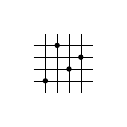
\begin{tikzpicture}[scale=0.15]
    \fill[white] (-.5,-.5) rectangle (5.5,5.5);
    \foreach \x in {1,...,4} {
        \draw[ultra thin] (\x,0)--(\x,5); %vline
        \draw[ultra thin] (0,\x)--(5,\x); %hline
    }
    \draw[fill=black] (1,1) circle (5pt);
    \draw[fill=black] (2,4) circle (5pt);
    \draw[fill=black] (3,2) circle (5pt);
    \draw[fill=black] (4,3) circle (5pt);
\end{tikzpicture}
}

\newcommand{\sB}{
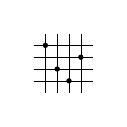
\begin{tikzpicture}[scale=0.15]
    \fill[white] (-.5,-.5) rectangle (5.5,5.5);
    \foreach \x in {1,...,4} {
        \draw[ultra thin] (\x,0)--(\x,5); %vline
        \draw[ultra thin] (0,\x)--(5,\x); %hline
    }
    \draw[fill=black] (1,4) circle (5pt);
    \draw[fill=black] (2,2) circle (5pt);
    \draw[fill=black] (3,1) circle (5pt);
    \draw[fill=black] (4,3) circle (5pt);
\end{tikzpicture}
}

\newcommand{\sC}{
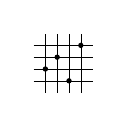
\begin{tikzpicture}[scale=0.15]
    \fill[white] (-.5,-.5) rectangle (5.5,5.5);
    \foreach \x in {1,...,4} {
        \draw[ultra thin] (\x,0)--(\x,5); %vline
        \draw[ultra thin] (0,\x)--(5,\x); %hline
    }
    \draw[fill=black] (1,2) circle (5pt);
    \draw[fill=black] (2,3) circle (5pt);
    \draw[fill=black] (3,1) circle (5pt);
    \draw[fill=black] (4,4) circle (5pt);
\end{tikzpicture}
}

\newcommand{\sD}{
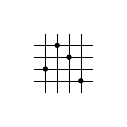
\begin{tikzpicture}[scale=0.15]
    \fill[white] (-.5,-.5) rectangle (5.5,5.5);
    \foreach \x in {1,...,4} {
        \draw[ultra thin] (\x,0)--(\x,5); %vline
        \draw[ultra thin] (0,\x)--(5,\x); %hline
    }
    \draw[fill=black] (1,2) circle (5pt);
    \draw[fill=black] (2,4) circle (5pt);
    \draw[fill=black] (3,3) circle (5pt);
    \draw[fill=black] (4,1) circle (5pt);
\end{tikzpicture}
}

\newcommand{\sE}{
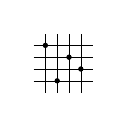
\begin{tikzpicture}[scale=0.15]
    \fill[white] (-.5,-.5) rectangle (5.5,5.5);
    \foreach \x in {1,...,4} {
        \draw[ultra thin] (\x,0)--(\x,5); %vline
        \draw[ultra thin] (0,\x)--(5,\x); %hline
    }
    \draw[fill=black] (1,4) circle (5pt);
    \draw[fill=black] (2,1) circle (5pt);
    \draw[fill=black] (3,3) circle (5pt);
    \draw[fill=black] (4,2) circle (5pt);
\end{tikzpicture}
}

\newcommand{\sF}{
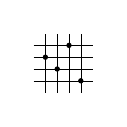
\begin{tikzpicture}[scale=0.15]
    \fill[white] (-.5,-.5) rectangle (5.5,5.5);
    \foreach \x in {1,...,4} {
        \draw[ultra thin] (\x,0)--(\x,5); %vline
        \draw[ultra thin] (0,\x)--(5,\x); %hline
    }
    \draw[fill=black] (1,3) circle (5pt);
    \draw[fill=black] (2,2) circle (5pt);
    \draw[fill=black] (3,4) circle (5pt);
    \draw[fill=black] (4,1) circle (5pt);
\end{tikzpicture}
}

\newcommand{\sG}{
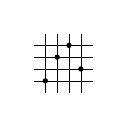
\begin{tikzpicture}[scale=0.15]
    \fill[white] (-.5,-.5) rectangle (5.5,5.5);
    \foreach \x in {1,...,4} {
        \draw[ultra thin] (\x,0)--(\x,5); %vline
        \draw[ultra thin] (0,\x)--(5,\x); %hline
    }
    \draw[fill=black] (1,1) circle (5pt);
    \draw[fill=black] (2,3) circle (5pt);
    \draw[fill=black] (3,4) circle (5pt);
    \draw[fill=black] (4,2) circle (5pt);
\end{tikzpicture}
}

\newcommand{\sH}{
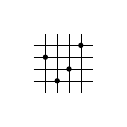
\begin{tikzpicture}[scale=0.15]
    \fill[white] (-.5,-.5) rectangle (5.5,5.5);
    \foreach \x in {1,...,4} {
        \draw[ultra thin] (\x,0)--(\x,5); %vline
        \draw[ultra thin] (0,\x)--(5,\x); %hline
    }
    \draw[fill=black] (1,3) circle (5pt);
    \draw[fill=black] (2,1) circle (5pt);
    \draw[fill=black] (3,2) circle (5pt);
    \draw[fill=black] (4,4) circle (5pt);
\end{tikzpicture}
}

\begin{tabular}{c|c|c|c|c|c}
    \adjustbox{valign=T}{$\textsf{sym}_0$} & \adjustbox{valign=T}{$\pi$} & \adjustbox{valign=T}{Rotate $0^\circ$} & \tsquare{A}{B}{C}{D} & \adjustbox{valign=T}{$1423$} & \adjustbox{valign=t}{\sA} \\
    \hline
    \adjustbox{valign=T}{$\textsf{sym}_1$} & \adjustbox{valign=T}{$\textsf{r}(\textsf{i}(\pi))$} & \adjustbox{valign=T}{Rotate $90^\circ$} & \tsquare{D}{A}{B}{C} & \adjustbox{valign=T}{$4213$} & \adjustbox{valign=t}{\sB}\\
    \hline
    \adjustbox{valign=T}{$\textsf{sym}_2$} & \adjustbox{valign=T}{$\textsf{i}(\textsf{r}(\textsf{i}(\textsf{r}(\pi))))$} & \adjustbox{valign=T}{Rotate $180^\circ$} & \tsquare{C}{D}{A}{B} & \adjustbox{valign=T}{$2314$} &\adjustbox{valign=t}{\sC} \\
    \hline
    \adjustbox{valign=T}{$\textsf{sym}_3$} & \adjustbox{valign=T}{$\textsf{i}(\textsf{r}(\pi))$} & \adjustbox{valign=T}{Rotate $270^\circ$} & \tsquare{B}{C}{D}{A} & \adjustbox{valign=T}{$2431$} & \adjustbox{valign=t}{\sD}\\
    \hline
    \adjustbox{valign=T}{$\textsf{sym}_4$} & \adjustbox{valign=T}{$\textsf{i}(\textsf{r}(\textsf{i}(\pi)))$} & \adjustbox{valign=T}{Horizontal flip} & \tsquare{D}{C}{B}{A} & \adjustbox{valign=T}{$4132$} &\adjustbox{valign=t}{\sE}\\
    \hline
    \adjustbox{valign=T}{$\textsf{sym}_5$} & \adjustbox{valign=T}{$\textsf{r}(\pi)$} & \adjustbox{valign=T}{Vertical flip} & \tsquare{B}{A}{D}{C} & \adjustbox{valign=T}{$3241$} &\adjustbox{valign=t}{\sF}\\
    \hline
    \adjustbox{valign=T}{$\textsf{sym}_6$} & \adjustbox{valign=T}{$\textsf{i}(\pi)$} & \adjustbox{valign=T}{Diagonal flip} & \tsquare{C}{B}{A}{D} & \adjustbox{valign=T}{$1342$} &\adjustbox{valign=t}{\sG}\\
    \hline
    \adjustbox{valign=T}{$\textsf{sym}_7$} & \adjustbox{valign=T}{$\textsf{r}(\textsf{i}(\textsf{r}(\pi)))$} & \adjustbox{valign=T}{Antidiagonal flip} & \tsquare{A}{D}{C}{B} & \adjustbox{valign=T}{$3124$} &\adjustbox{valign=t}{\sH}\\
\end{tabular}

}